\documentclass{article}

\usepackage{amsmath,amssymb}
\usepackage{ntheorem}
%\usepackage{amsthm}
\theoremstyle{break}
\newtheorem*{theorem}{Theorem}

\usepackage{tikz}
\usetikzlibrary{shapes,snakes}
\usetikzlibrary{matrix}
\usetikzlibrary{calc}
\usetikzlibrary{positioning}

\title{Orthogonal Projections Notes}
\author{David E. James}

\begin{document}

\maketitle
Orthogonal Projections

\bigskip

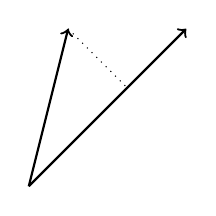
\begin{tikzpicture}
\coordinate (A) at (0,0);
\coordinate (B) at (2,2);
\coordinate (C) at (0.5,2);

\draw[->, thick] (A) -- (B);
\draw[->, thick] (A) -- (C);
\draw[dotted] (C) -- ($(A)!(C)!(B)$);
\end{tikzpicture}

\bigskip

Goal: if W is a subspace in $\mathbb{R}^n$, how do we get $\hat{y}$, the
projection in W of $\vec{y}$?
\begin{equation}
    \hat{y} = \text{proj}_W(\vec{y})
\end{equation}

\bigskip

\begin{theorem}[Orthogonal Decomposition Theorem]
Let W be a subspace with orthogonal basis $\{\vec{u_1} \dotsm \vec{u_p}\}$.
Let $\vec{y} \in \mathbb{R}^n$.
\begin{align}
    \hat{y} = \left(\frac{\vec{y} \cdot \vec{u}_1}{\vec{u}_1 \cdot \vec{u}_1}\right)\vec{u}_1 \dotsm \left(\frac{\vec{y} \cdot \vec{u}_p}{\vec{u}_p \cdot \vec{u}_p}\right)\vec{u}_p
\end{align}

decompose...

\begin{align}
    \vec{y} = \hat{y} + \left( \vec{y} - \hat{y} \right) \\
    \hat{y} \in W \\
    \left( \vec{y} - \hat{y} \right) \in W^{\perp}
\end{align}

\end{theorem}




\begin{theorem}[Best Approximation Theorem]
    Let W be a subspace of $\mathbb{R}^n$, $\vec{y} \in \mathbb{R}^n$, $\hat{y} = \text{proj}_W(\vec{y})$
    \bigskip
    \begin{equation}
        \text{Then } \hat{y} \text{ is the closest point in W to }\vec{y}.
    \end{equation}
    and...
    \begin{equation}
        \text{If } \vec{y} \in W \text{ then } \hat{y} = \vec{y}
    \end{equation}


\end{theorem}


\begin{theorem}[Projection is a Linear Transform]
Let W be a subspace in $\mathbb{R}^n$ \\
Let $\{\vec{u}_1 \dotsm \vec{u}_p \}$ be an orthonormal basis of W

\medskip

Orthonormal basis means $\vec{u}_i$ are all unit vectors, so:
\begin{equation}
    \lvert\vec{u}_1\rvert = 1\text{ and } \vec{u}_1 \cdot \vec{u}_1 = 1
\end{equation}

\end{theorem}



\end{document}
